\documentclass{article}
\usepackage{graphicx}
\title{Heart Dataset representation by graphs}

\begin{document}
	\maketitle
	\begin{figure}[h]
		\centering
		\caption{\label{4a}Gender wise heart disease distribution}
		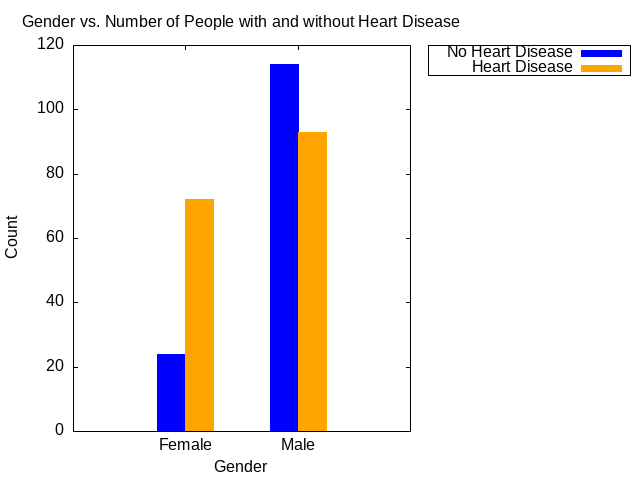
\includegraphics[scale=0.7]{4a.png}
	\end{figure}
	
	\begin{figure}[h]
		\centering
		\caption{\label{4b}Correlation between Age and blood pressure}
		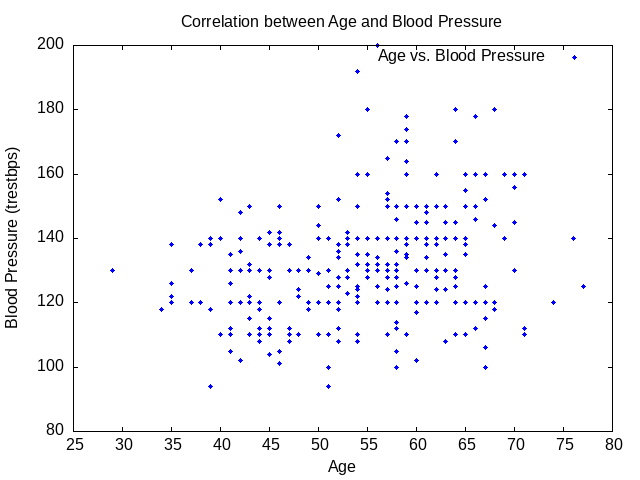
\includegraphics[scale=0.7]{4b.png}
	\end{figure}
	\begin{figure}[h]
		\centering
		\caption{\label{4c}Age vs Cholestrol distribution people not have heart disease}
		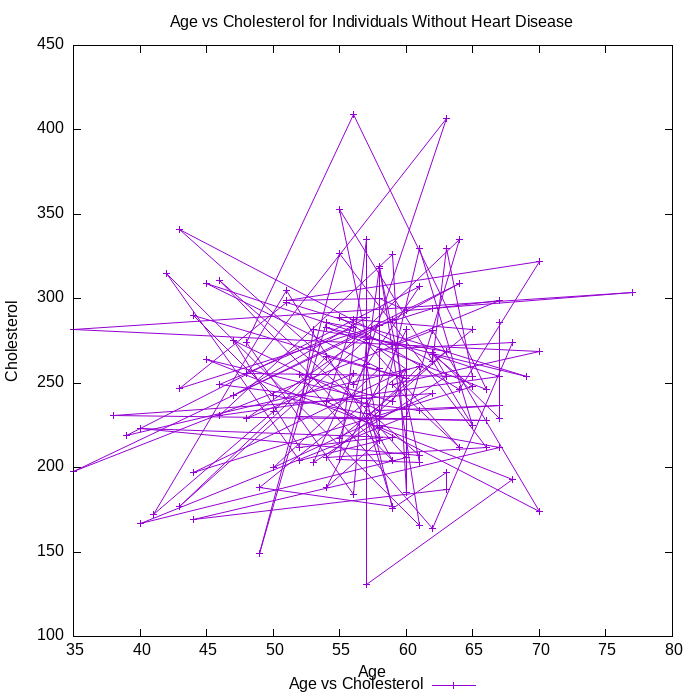
\includegraphics[scale=0.7]{4c.png}
	\end{figure}
	\begin{figure}[h]
		\centering
		\caption{\label{4d}Pie chart Distribution of Heart disease (Age wise)}
		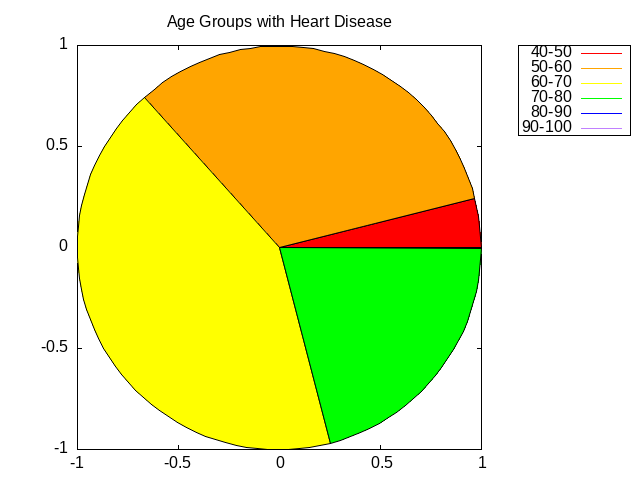
\includegraphics[scale=0.7]{4d.png}
	\end{figure}
\end{document}